\documentclass{article}
\sloppy
%\usepackage[margin=0.5in]{geometry}
%\usepackage[landscape,margin=0.5in]{geometry}
\usepackage[landscape,top=-1in,left=0.5in,right=0.5in,bottom=0.0in]{geometry}
\usepackage{graphicx}
\usepackage{multicol}
\usepackage{overpic}
\usepackage{hyperref}

\usepackage{fancyvrb}
\setlength{\parindent}{0in}


\newcommand{\nop}[1]{}
\newcommand{\myfig}[1]{\newpage\begin{overpic}[scale=1.5]{figures/#1}}
\newcommand{\myfigs}[2]{\newpage\begin{overpic}[scale=#1]{figures/#2}}
\newcommand{\myfigsp}[3]{\newpage\begin{overpic}[scale=#1,page=#2]{figures/#3}}
\newcommand{\myfigend}{\end{overpic}}
\newcommand{\myput}[2]{\put(10,#1){$\bullet$ #2}}
\newcommand{\myputn}[2]{\put(15,#1){#2}}

\newcommand{\bi}{\begin{itemize}}
\newcommand{\ii}{\item}
\newcommand{\ei}{\end{itemize}}
\newcommand{\ti}[1]{
\newpage
\mbox{~}

\vspace{1.25in}
\centerline{\bf #1}
}

\newcommand{\la}{\ensuremath{\langle}}
\newcommand{\ra}{\ensuremath{\rangle}}


\RecustomVerbatimEnvironment
  {Verbatim}{Verbatim}
  {frame=single,commandchars=\\\{\}}

\begin{document}


\huge\sf

\ti{RPC and Rendezvous}
\centerline{Andrews, Chapter 08}
\bi
\ii Message passing:
\bi
  \ii Best for filters and interacting peers.
  \ii Clients and servers require two messages.
  \ii Each client needs a different reply channel.
  \ii Can lead to large number of channels.
\ei
\ii RPC and rendezvous best for client/servers:
\bi
\ii Combine aspects of monitors and synchronous message passing.
\ii Call and return like message passing.
\ii Caller delays until return like monitor calls.
\ei
\ii RPC:
\bi
\ii Create a new process for each call.
\ei
\ii Rendezvous:
\bi
\ii Call to an existing process.
\ei
\ei

\ti{RPC \hspace{5in} Rendezvous}

\vspace{1cm}

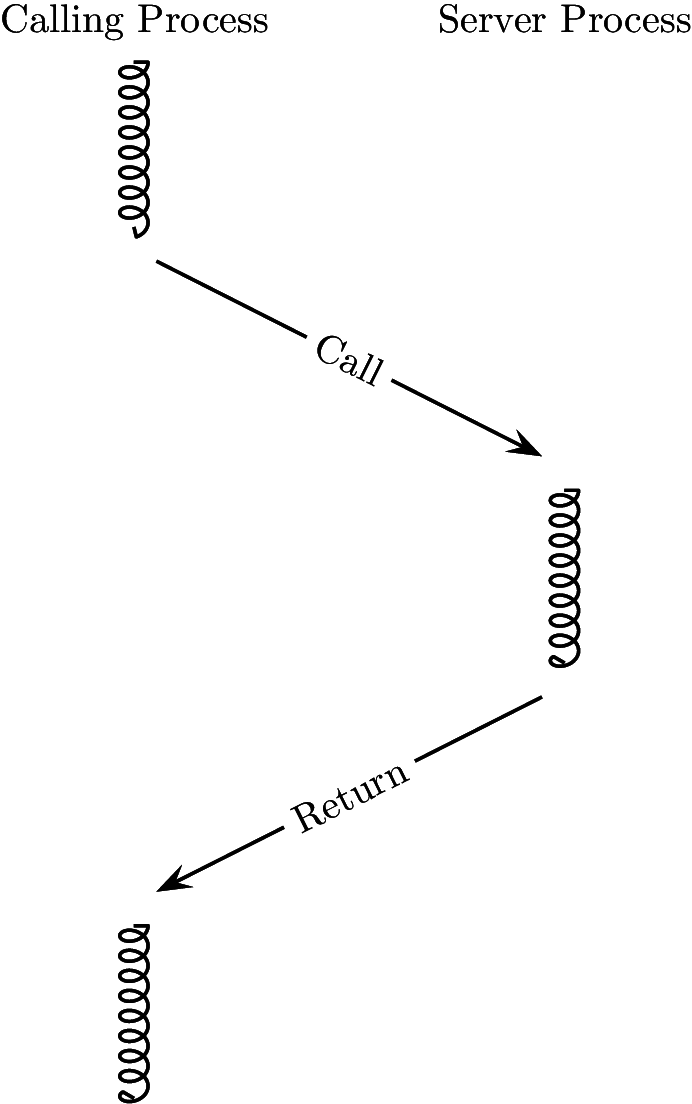
\includegraphics[scale=0.4]{figures/rpc.png}\hfill
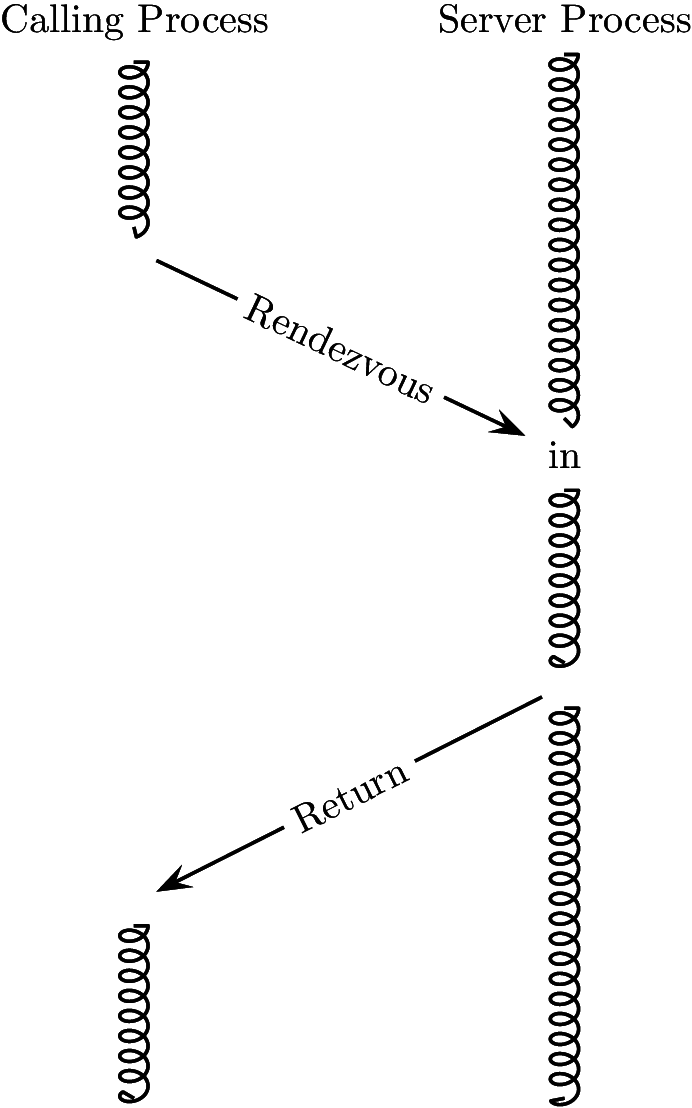
\includegraphics[scale=0.4]{figures/rendezvous.png}

\nop{
\myfig{timing_rpc_rend.pdf}
\myfigend
}

\ti{RPC {\em vs.} Monitors}
\bi
\ii Monitors:
\bi
\ii Monitors have two kinds of components:  processes and monitors.
\ii Processes communicate and synchronize by calling monitor procedures.
\ii Processes and monitors are all in the same address space.
\ei
\ii RPC:
\bi
\ii One program component: the module.
\ii Modules have both processes and procedures.
\ii Modules reside in different address spaces ({\em e.g.} nodes in a
network). 
\ei
\ei

\nop{
\myfig{modules.pdf}
\myfigend
}

\ti{Modules}
\begin{Verbatim}
module mname
  \mbox{\rm headers of exported operations};
body
  \mbox{\rm variable declarations};
  \mbox{\rm initialization code};
  \mbox{\rm procedures for exported operations};
  \mbox{\rm local procedures and processes};
\end{Verbatim}
\bi
\ii Local processes are called {\em background processes}
\ii The header of an operation {\tt opname} is specified with {\tt
  op}:
\begin{Verbatim}
op opname(\mbox{\rm formals}) [returns \mbox{\rm result}]
\end{Verbatim}
\ii The operation itself is implemented by {\tt proc}:
\begin{Verbatim}
proc opname(\mbox{\rm formal identifiers}) returns \mbox{\rm result identifier}
  \mbox{\rm declarations of local variables};
  \mbox{\rm statements};
end
\end{Verbatim}
\ii A process in one module calls a procedure in another module with:
\begin{Verbatim}
call mname.opname(\mbox{\rm arguments})
\end{Verbatim}
\ei

\ti{RPC}
\begin{multicols}{2}
\bi
\ii A {\em new process} services the call.
\ii Arguments are passed as messages.
\ii The calling process delays during the call.
\ii When the call returns it sends results as a message and
terminates.
\ii After receiving results, the calling process continues.
\ei
\vfill
\columnbreak
\hfill
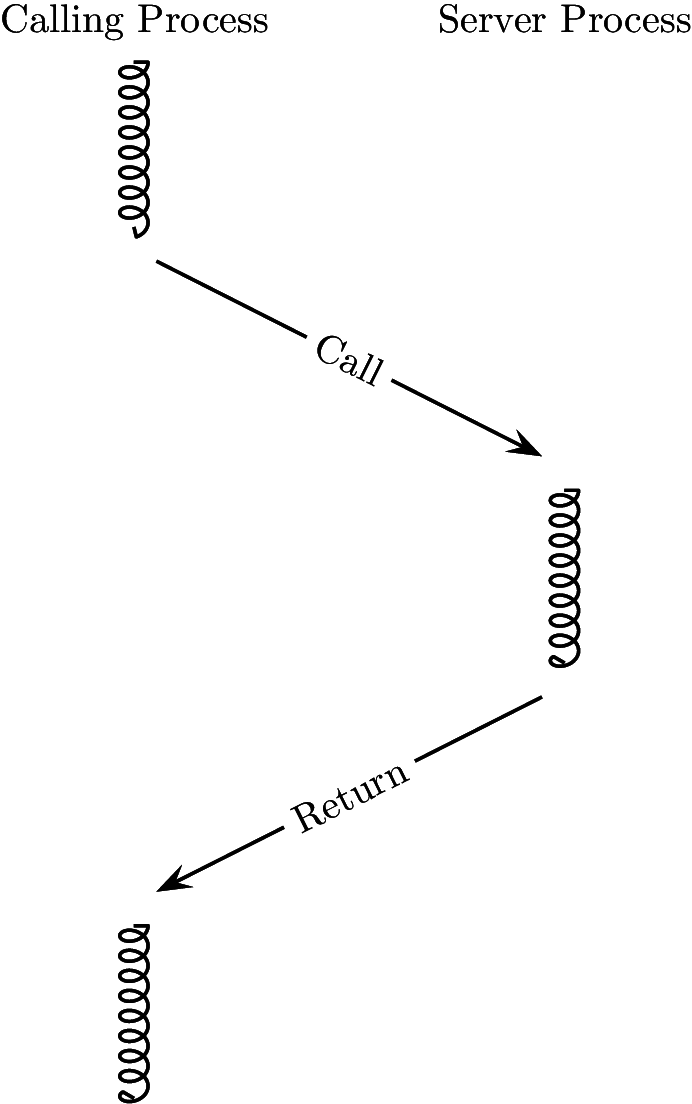
\includegraphics[scale=0.4]{figures/rpc.png}
\end{multicols}

\ti{Synchronization in Modules}
\bi
\ii Synchronization between caller and server is implicit.
\ii From client appears as normal procedure call.
\ii Need mutually exclusive access for more than one call to the
server and background processes.  Two approaches:
\bi
\ii All server processes are mutually exclusive (similar to
monitors).  Can use semaphores or condition variables for other
synchronization. 
\ii Server processes execute concurrently.  Need to explicitly program 
both mutual exclusion and synchronization.  Can use any of the methods
discussed in the book.
\ei
\ii The first approach is simpler to implement and program with.
\ii The second approach is more general and fits better with modern
architectures, which are multi-core.
\ii The text assumes the second approach.  All RPC modules will have
explicit synchronization programmed.
\ei




\myfigs{1.25}{8_1.pdf}
\myfigend
\myfig{8_2a.pdf}
\myfigend
\myfigs{1.3}{8_2b.pdf}
\myfigend
\myfigs{1.2}{8_3.pdf}
\myfigend
\myfig{8_4.pdf}
\myfigend

\ti{Rendezvous}
\begin{multicols}{2}
\bi
\ii Rendezvous combines communication and synchronization.
\ii Clients invoke operations with {\tt call}
\ii A server process uses an {\em input statement} to wait for and
handle the call. 
\ii Operations are not handled concurrently.
\ei
\vfill
\columnbreak
\hfill
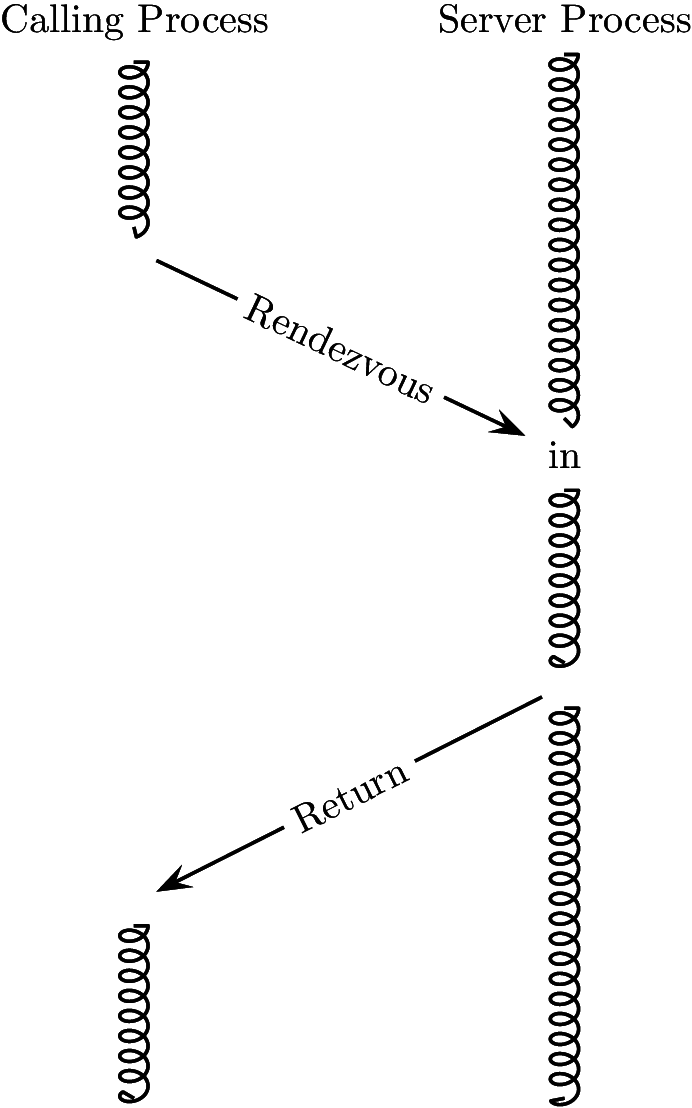
\includegraphics[scale=0.4]{figures/rendezvous.png}
\end{multicols}

\nop{
\myfig{operations.pdf}
}

\ti{Input Statements}

\begin{Verbatim}[commandchars=\\\{\}]
in op1(formals1) and B1 by e1 -> S1;
[] op2(formals2) and B2 by e2 -> S1;
...
[] opN(formalsN) and BN by eN -> SN;
ni
\end{Verbatim}
\bi
\ii Provided by {\bf Ada} in slightly modified form.
\ii Part before the {\tt ->} is the {\bf guard}
\ii {\tt opi} is the name of the operation
\ii {\tt Bi} is the {\bf synchronization expression}
\bi\ii boolean determines if this branch is open\ei
\ii {\tt ei} is the {\bf scheduling expression}
\bi\ii number determines priority\ei
\ei

\ti{Input Statements}

\begin{Verbatim}[commandchars=\\\{\}]
in op1(formals1) and B1 by e1 -> S1;
[] op2(formals2) and B2 by e2 -> S1;
...
[] opN(formalsN) and BN by eN -> SN;
ni
\end{Verbatim}
\bi
\ii A guard {\bf succeeds} when
\begin{enumerate}
\ii the operation has been called
\ii the synchronization expression is true (or omitted)
\end{enumerate}
\ii The boolean can depend on the parameters (not true in Ada).
\ii Execution of {\tt in} delays until some guard succeeds.
\ii If more than one guard succeeds the {\tt in} statement services
the oldest.
\ii If scheduling expressions are present, oldest of minimum.
\ii Synchronization and scheduling expressions also present in some
message-passing systems, {\em e.g.} MPI.
\ei

\myfig{8_5.pdf}
\myfigend
\myfig{8_6.pdf}
\myfigend
\myfig{8_7.pdf}
\myfigend
\myfig{8_8.pdf}
\myfigend
\myfig{8_9.pdf}
\myfigend
\myfig{8_10.pdf}
\myfigend

\ti{Skipping \S 8.3 and \S 8.4}
\nop{
\myfig{table.pdf}
\myfigend
\myfig{8_11.pdf}
\myfigend
\myfig{8_12.pdf}
\myfigend
\myfig{8_13.pdf}
\myfigend
\myfig{8_14.pdf}
\myfigend
\myfigsp{1}{1}{8_15.pdf}
\myfigend
\myfigsp{1}{2}{8_15.pdf}
\myfigend
}

\myfigsp{1}{1}{8_16.pdf}
\put(70,70){$\bullet$ Java {\tt rmi} library}
\myfigend
\myfigsp{1}{2}{8_16.pdf}
\myfigend

\ti{Tasks, Rendezvous, and Protected Types in Ada}
\bi
\ii \url{http://en.wikibooks.org/wiki/Ada_Programming/Tasking}
\ei

\myfig{ada_tasks.pdf}
\myfigend

\myfig{ada_accept_select.pdf}
\myfigend

\myfig{ada_protected_types.pdf}
\myput{58}{Similar to Monitors}
\myput{56}{At most one task executes a protected procedure at a time.}
\myput{54}{Caller waits until it can have access {\em and} the guard is true.}
\myput{52}{{\tt requeue} puts the task back on the calling queue.}
\myfigend


\myfig{8_17.pdf}
\put(11,75){\LARGE\tt entry}
\put(14.8,75.25){\rule{3.25cm}{1pt}}
\myput{46}{{\tt requeue} statement defers completion of the call.}
\myput{44}{Is it reusable?}
\myfigend

\myfigs{1.3}{8_18.pdf}
\myfigend
\myfigs{1.2}{8_19.pdf}
\myfigend

\myfig{8_6.pdf}
\myfigend




\ti{Skipping \S 8.7}
\centerline{The SR Language}
\nop{
\myfig{sr_resources.pdf}
\myfigend
\myfig{8_20.pdf}
\myfigend
}

\end{document}